
\section{Kittel \& Kroemer: Chapter 1 and 2}
Derives statistical mechanics from the fundamental assumption. The assumption is: \emph{Every particular state of a system is occupied with equal probability}. The number of available states with a given energy implies the maximum entropy principle. 
\begin{itemize}
    \item Accessible states: $g(N,U)$
    \item For multiple systems put together: $g = g_1 \cdot ... \cdot g_n$
    \item Entropy: $S=k_B \sigma = k_B \log{g}$
    \item Temperature: $\tau = k_B T = (\partial U/ \partial \sigma)_{N,V}$
\end{itemize}


\section{Callen: Chapter 1}
Goes over the very basics and tries to build an intuitive relationship between energy and entropy and other extensive parameters.
\begin{itemize}
    \item \textbf{Postulate I.} \emph{There exist particular states (called equilibrium states) of simple systems that, macroscopically, are characterized completely by internal energy U, the volume V, and the mole numbers N.}
    \item \textbf{Postulate II.} \emph{There exists a function (called the entropy S) of the extensive parameters of any composite system, defined for all equilibrium states and having the following property: The values assumed by the extensive parameters in the absence of an internal constraint are those that maximize the entropy over the manifold of constrained equilibrium states.}
    \item \textbf{Postulate III.} \emph{The entropy of a composite system is additive over the constituent subsystems. The entropy is continuous and differentiable and is a monotonically increasing function of energy.}
    \item \textbf{Postulate IV.} \emph{The entropy of any system vanishes in the state of zero temperature.}
\end{itemize}

Work and Heat: $dU = dQ + dW_M = TdS - PdV$

\section{Callen: Chapter 2}

Intensive parameters are those given by the partial derivatives of the fundamental relation. They are defined by the following:

\begin{align*}
    (\partial U/\partial S)_{V,N} & \equiv  T & (\partial S/\partial U)_{V,N} & \equiv  1/T \\ 
    (\partial U/\partial V)_{S,N} & \equiv -P & (\partial S/\partial V)_{U,N} & \equiv -P/T \\ 
    (\partial U/\partial N)_{S,V} & \equiv \mu & (\partial S/\partial N)_{U,V} & \equiv \mu/T
\end{align*}
\begin{equation}
    dU = TdS-PdV+\mu dN
\end{equation}
\begin{equation}
    dS = \frac{1}{T} dU + \frac{P}{T} dV - \frac{\mu}{T} dN
\end{equation}
The chapter also goes over the conditions for equilibrium with heat flow, mechanical equilibrium, and equilibrium with matter flow. These are rather straightforward to derive, so they are omitted. (\emph{Note: Stoichiometry is important when dealing with chemical equilibrium.})

\section{Callen: Chapter 3}
Goes over Euler and Gibbs-Duhem relation then summarizes information about the fundamental relation. The chapter then covers ideal gases, Van der Waals fluid, radiation, and the rubber band. The last section goes over the preferred derivatives briefly ($\alpha, c_p, \kappa_T$).
\begin{itemize}
    \item Euler Relation: $U=TS-PV+\mu N$
    \item Gibbs-Duhem Relation: relations among the derivatives of U. The one for single-component system is $0 = S dT - V dP + N d\mu $
    \item The fundamental relation contains all information about a thermodynamic system.
    \item Two equations of state [such as T,P] can determine the fundamental relation with an unknown constant using the Gibbs-Duhem relation.
    \item NOTE: The potentials given by Legendre Transformations are not fundamental relations!
\end{itemize}


\section{Callen: Chapter 4}
Covers possible processes, quasi-static processes, reversible processes, maximum work theorem, Carnot cycle, refrigeration, and Otto cycle.

\begin{itemize}
    \item A process is possible if and only if $\Delta S \geq 0$ and the laws of mechanics are obeyed.
    \item Quasi-Static Process: idealized process where each state can be represented with the fundamental relation as an equilibrium state.
    \item There is a relaxation time $\tau$ between equilibrium states, which is the limit for a process to be \emph{quasi-static}. (Usually related to the speed of sound.)
    \item Reversible Process: $\delta S_{Total}=0$ \emph{Note: Subsystems must still maximize entropy.}
    \item Maximum Work Theorem: reversible process with work extracted from the heat transferred between subsystems
    \item See \emph{Figure 4.6} on page 115 for diagrams of engine, refrigerator, and heat pump.
\end{itemize}

\textbf{Carnot Cycle:}\footnote{I suggest googling this and reading wikipedia or another source.} A hot reservoir and cold reservoir are put into contact with a reversible work source. The following cycle is done:

\begin{enumerate}
    \item Isothermal expansion
    \item Isentropic (reversible adiabatic) expansion
    \item Isothermal compression
    \item Adiabatic reversible compression
\end{enumerate}
\begin{figure}[h]
    \centering
    \begin{minipage}{.5\textwidth}
      \centering
      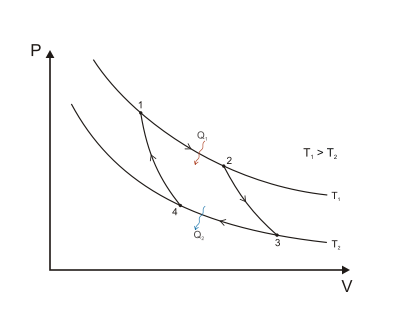
\includegraphics[width=.6\linewidth]{Images/Carnot_P-V.png}
      \captionof{figure}{Carnot Cycle Pressure-Volume Plot}
      \label{fig:test1}
    \end{minipage}%
    \begin{minipage}{.5\textwidth}
      \centering
      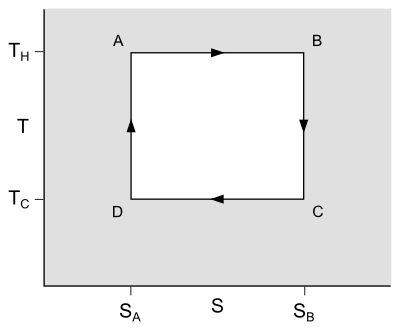
\includegraphics[width=.6\linewidth]{Images/Carnot_T-S.png}
      \captionof{figure}{Carnot Cycle Temperature-Entropy Plot}
      \label{fig:test2}
    \end{minipage}
\end{figure}
\begin{center}
\rule{.8\textwidth}{.5pt}
\end{center}
\textbf{Otto Cycle:} Idealized cycle of a typical spark ignition piston engine often used in automobile engines. The following image sums it up:
\begin{figure}[ht]
    \centering
    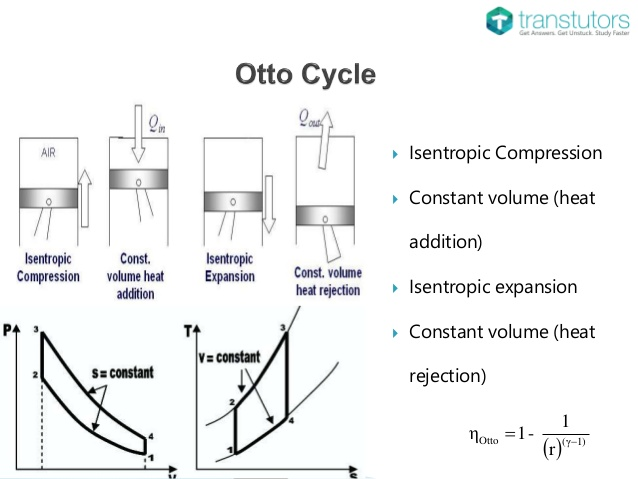
\includegraphics[scale=.4]{Images/otto-cycle.jpg}
    \caption{Otto Cycle Summary}
    \label{fig:otto}
\end{figure}

\section{Callen: Chapter 5}
Covers the Energy Minimum Principle, Legendre Transformations, and the resulting potentials. These are developed because experimentation usually finds the intensive parameters easier to measure. The book also briefly goes over Massieu Functions (Legendre Transformations of the entropy), but this was not covered in class.

\textbf{Energy Minimum Principle:} The Entropy Maximum Principle implies a corollary principle for the minimization of internal energy in a system.

\textbf{Legendre Transformations:} The process replaces a number of the function's variables with the partial derivatives in those variables. 

\begin{center}
    \rule{.8\textwidth}{.5pt}
    
    \textbf{Helmholtz Potential or Free Energy}
    
    $F \equiv U - TS \implies dF = -SdT - PdV + \mu_1dN_1 + \mu_2dN_2 + ... $
    \rule{.8\textwidth}{.5pt}
\end{center}
\begin{tabularx}{\textwidth}{X | X}
    {\begin{align*}
        & U = U(S,V,N_1,N_2,...) \\
        & T = \partial U/\partial S \\
        & F = U - TS \\
        & \text{Elimination of U and S} \\
        & F = F(T,V,N_1,N_2,...)
    \end{align*}} 
    & 
    {\begin{align*}
        & F=F(T,V,N_1,N_2,...) \\
        & -S = \partial F/\partial T \\
        & U = F + TS \\
        & \text{Elimination of F and T} \\
        & U = U(S,V,N_1,N_2,...)
    \end{align*}} 
\end{tabularx}
\begin{center}
    \rule{.8\textwidth}{.5pt}
    
    \textbf{Enthalpy}
    
    $H \equiv U + PV \implies dH = TdS + VdP + \mu_1dN_1 + \mu_2dN_2 + ... $
    \rule{.8\textwidth}{.5pt}
\end{center}
\begin{tabularx}{\textwidth}{X | X}
    {\begin{align*}
        & U = U(S,V,N_1,N_2,...) \\
        & -P = \partial U/\partial V \\
        & H = U + PV \\
        & \text{Elimination of U and V} \\
        & H = H(S,P,N_1,N_2,...)
    \end{align*}} 
    & 
    {\begin{align*}
        & H=H(S,P,N_1,N_2,...) \\
        & V = \partial H/\partial P \\
        & U = H - PV \\
        & \text{Elimination of H and P} \\
        & U = U(S,V,N_1,N_2,...)
    \end{align*}} 
\end{tabularx}
\begin{center}
    \rule{.8\textwidth}{.5pt}
    
    \textbf{Gibbs Potential or Free Energy}
    
    $G \equiv U - TS + PV \implies dG = -SdT + VdP + \mu_1dN_1 + \mu_2dN_2 + ... $
    \rule{.8\textwidth}{.5pt}
\end{center}
\begin{tabularx}{\textwidth}{X | X}
    {\begin{align*}
        & U = U(S,V,N_1,N_2,...) \\
        & T = \partial U/\partial S \\
        & -P = \partial U/\partial V \\
        & G = U - TS + PV \\
        & \text{Elimination of U, V, and S} \\
        & G = G(T,P,N_1,N_2,...)
    \end{align*}} 
    & 
    {\begin{align*}
        & G=G(T,P,N_1,N_2,...) \\
        & -S = \partial G/\partial T \\
        & V = \partial G/\partial P \\
        & U = G + TS - PV \\
        & \text{Elimination of G, P, and T} \\
        & U = U(S,V,N_1,N_2,...)
    \end{align*}} 
\end{tabularx}
\newpage
\begin{center}
    \rule{.8\textwidth}{.5pt}
    
    \textbf{Grand-Canonical Potential}
    
    $U[T,\mu] \equiv U - TS - \mu N \implies dU = -SdT - PdV - Nd\mu$
    \rule{.8\textwidth}{.5pt}
\end{center}
\begin{tabularx}{\textwidth}{X | X}
    {\begin{align*}
        & U = U(S,V,N_1,N_2,...) \\
        & T = \partial U/\partial S \\
        & \mu = \partial U/\partial N \\
        & U[T,\mu] = U - TS - \mu N \\
        & \text{Elimination of U, N, and S} \\
        & U = U(T,P,\mu)
    \end{align*}} 
    & 
    {\begin{align*}
        & U = U(T,P,\mu) \\
        & -S = \partial U[T,\mu]/\partial T \\
        & -N = \partial U[T,\mu]/\partial \mu \\
        & U = U[T,\mu] + TS + \mu N \\
        & \text{Elimination of G, P, and T} \\
        & U = U(S,V,N)
    \end{align*}} 
\end{tabularx}



\section{Processes in Systems}

\begin{table}[!htbp]
    \caption{Types of Processes}
    \centering
        \begin{tabular}{c|c c}
            \toprule
            Name        & Meaning                  & Notes \\
            \midrule
            Adiabatic   & $\Delta N,\Delta Q = 0$  & \\
            Isobaric    & $\Delta P = 0$           & \\
            Isochoric   & $\Delta V = 0$           & \\
            Isothermal  & $\Delta T = 0$           & \\
            Isentropic  & $\Delta N, \Delta Q = 0$ & Also reversible \\
            Isenthalpic & $\Delta H = 0$           &
    \end{tabular}
    \label{tab:processes}
\end{table}

